% !TEX root = ../dg.tex

\section{Geodesics on Grassmannians}
\label{sec:geodesics on grassmannians}

The goal in this section is to describe geodesics on Grassmannians. This is knowledge that I have used many times in my research career; since Grassmannians pop up everywhere from string theory to random polygons to hyperspectral imaging to video analysis to algebraic geometry, you may find this information important at some point, too. The information in this section is mostly drawn from Edelman, Arias, and Smith's amazing paper~\cite{edelmanGeometryAlgorithmsOrthogonality1999}.

Recall from \Cref{sec:stiefel and grassmann} that the Grassmannian $\Gr(k,\R^n)$ is the collection of $k$-dimensional linear subspaces of $\R^n$, and that it can be realized as a quotient of $\orthog(n)$ by
\[
	\Gr(k,\R^n) \cong \orthog(n)/(\orthog(k) \times \orthog(n-k)).
\]

In other words, we can interpret points in the Grassmannian as equivalence classes $[Q]$ of all orthogonal matrices whose first $k$ columns span the same subspace as those of $Q \in \orthog(n)$. Concretely,
\[
	[Q] := \left\{ Q \begin{bmatrix} U_k & 0 \\ 0 & U_{n-k} \end{bmatrix} : U_k \in \orthog(k), U_{n-k} \in \orthog(n-k) \right\}.
\]
The tangent space $T_Q \orthog(n)$ splits into \emph{horizontal} and \emph{vertical} components: the vertical space is the subspace tangent to $[Q]$ (i.e., moving in those directions does not change the point on the Grassmannian), and the horizontal space is the orthogonal complement of the vertical space.

From the above description of $[Q]$, it should be pretty clear that the vertical space is
\[
	\left\{Q\begin{bmatrix} A & 0 \\ 0 & C \end{bmatrix} : A \text{ is $k \times k$ skew-symmetric and $C$ is $(n-k) \times (n-k)$ skew-symmetric}\right\}.
\] 
Hence, the horizontal space, which we can identify with $T_{[Q]} \Gr(k,\R^n)$, consists of matrices of the form
\[
	\Delta = Q \begin{bmatrix} 0 & -B^T \\ B & 0 \end{bmatrix},
\]
where $B$ is an arbitrary $(n-k) \times k$ matrix. Note that this immediately recovers the fact that $\dim(\Gr(k,\R^n)) = k(n-k)$.

We get the standard Riemannian metric on $\Gr(k,\R^n)$ by restricting the metric on $\orthog(n)$ to the horizontal space (it is also traditional to multiply by $1/2$ because of the repeated $B$'s in the expression for $\Delta$ above). So what is the metric on the orthogonal group?

We get a left-invariant metric on $\orthog(n)$ by pushing around any inner product we like on $T_I\orthog(n) \subset T_I \GL_n(\R) = \Mat_{n \times n}(\R)$, where the standard inner product is the Frobenius inner product
\[
	\langle M_1, M_2 \rangle_{\text{Fr}} = \tr(M_1^T M_2).
\]
When we restrict this to $T_I\orthog(n)$, which consists of the skew-symmetric $n \times n$ matrices, we see that
\begin{multline*}
	\langle [X,Y],Z \rangle_{\text{Fr}} = \tr([X,Y]^TZ)= \tr((XY-YX)^TZ) = \tr(Y^TX^TZ-X^TY^TZ) = \tr(Y^TX^TZ - Y^TZX^T) \\
	= \tr(-Y^TXZ +Y^TZX) = \tr(Y^T[Z,X]) = \langle Y, [Z,X]\rangle_{\text{Fr}}
\end{multline*}
using cyclic invariance of the trace and the fact that $X^T = -X$. Therefore, \Cref{thm:bi-invariant metric condition} implies that the left-invariant metric $g_{\orthog(n)}$ on $\orthog(n)$ induced by $\langle \cdot , \cdot \rangle_{\text{Fr}}$ is bi-invariant.

What is this metric? First, recall that, for $Q \in \orthog(n)$, $T_Q \orthog(n) = \{Q X : X \text{ is skew-symmetric}\}$ since $T_I \orthog(n)$ consists of skew-symmetric matrices and $(dL_Q)_I X = QX$. Then, for $QX,QY \in T_Q \orthog(n)$,
\[
	g^{\orthog(n)}_Q(QX,QY) = \langle (dL_{Q^{-1}})_Q QX, dL_{Q^{-1}})_Q QY \rangle_{\text{Fr}} = \langle Q^{-1}QX, Q^{-1}QY \rangle_{\text{Fr}} = \langle X, Y \rangle_{\text{Fr}} = \tr(X^TY).
\]
Note that this is really just the Frobenius inner product of $QX$ with $QY$: 
\[
	\langle QX, QY \rangle_{\text{Fr}} = \tr((QX)^T(QY)) = \tr(X^T Q^T Q Y) = \tr(X^TY).
\]

Therefore, with the factor of $1/2$ mentioned previously, the induced metric on $\Gr(k, \R^n)$ is given by, for $\Delta_i = Q\begin{bmatrix} 0 & -B_i^T \\ B_i & 0 \end{bmatrix} \in T_{[Q]}\Gr(k,\R^n)$,
\[
	g_{[Q]}(\Delta_1,\Delta_2) = \frac{1}{2}\tr\left(\begin{bmatrix} 0 & B_1^T \\ -B_1 & 0 \end{bmatrix} \begin{bmatrix} 0 & -B_2^T \\ B_2 & 0 \end{bmatrix}\right) = \frac{1}{2} \tr(B_1^TB_2 + B_1B_2^T) = \tr(B_1^TB_2)
\]

From \Cref{thm:bi-invariant exp} we know that geodesics on $\orthog(n)$ take the form $\gamma(t) = Q e^{tX}$ where $Q \in \orthog(n)$, $X$ is skew-symmetric, and we have $\gamma(0) = Q$ and $\gamma'(0) = QX \in T_Q \orthog(n)$. 

If $Q \in \orthog(n)$ and $\Delta = Q\begin{bmatrix} 0 & -B^T \\ B & 0 \end{bmatrix} \in T_{[Q]}\Gr(k,\R^n)$, then 
\[
	\gamma(t) = Q e^{t{\tiny\begin{bmatrix} 0 & -B^T \\ B & 0 \end{bmatrix}}}
\]
is a horizontal curve: the velocity vector $\gamma'(t) = Q e^{t{\tiny\begin{bmatrix} 0 & -B^T \\ B & 0 \end{bmatrix}}} \begin{bmatrix} 0 & -B^T \\ B & 0 \end{bmatrix}$ is in the horizontal space at $\gamma(t) = Qe^{t {\tiny\begin{bmatrix} 0 & -B^T \\ B & 0 \end{bmatrix}}}$. This means that $[\gamma(t)]$ is a geodesic in the Grassmannian, and conversely it can be shown that every geodesic in $\Gr(k,\R^n)$ has a horizontal lift of this form.

In general, when we're working with the Grassmannian, we'd rather avoid working with $n \times n$ matrices (especially when $k$ is much smaller than $n$). Since we also know that $\Gr(k,\R^n) = \St(k,\R^n)/\orthog(k)$, we can also represent points in the Grassmannian by equivalence classes of $n \times k$ matrices $Y$ with orthonormal columns:
\[
	[Y] = \{Y U_k : U_k \in \orthog(k)\}.
\]
In practice, we can just think of $Y$ as the first $k$ columns of the orthogonal matrix $Q$ from before. The above expression makes it clear that the vertical space of the projection $\St(k,\R^n) \to \Gr(k,\R^n) = \St(k,\R^n)/\orthog(k)$ consists of $n \times k$ matrices of the form
\[
	Y A,
\]
where $A$ is $k \times k$ skew-symmetric; that is, it corresponds to infinitesimal rotations of the basis for the subspace given by the columns of $Y$. Therefore, the horizontal space, which we can identify with $T_{[Y]} \Gr(k,\R^n)$, consists of all $n \times k$ matrices $H$ whose columns are perpendicular to the column space of $Y$; that is,
\[
	Y^T H = 0.
\]
Here's another way to see this: if $Y$ consists of the first $k$ columns of an orthogonal matrix $Q = \begin{bmatrix} Y & Z \end{bmatrix}$, then the first $k$ columns of 
\[
	Q \begin{bmatrix} 0 & -B^T \\ B & 0 \end{bmatrix} = \begin{bmatrix} Y & Z \end{bmatrix} \begin{bmatrix} 0 & -B^T \\ B & 0 \end{bmatrix} = \begin{bmatrix} ZB & -YB^T \end{bmatrix}
\]
are $H = ZB$, and, since the columns of $Y$ are perpendicular to the columns of $Z$,
\[
	Y^T H = Y^T ZB = 0.
\]

In terms of $n \times k$ matrices, the Riemannian metric on the Grassmannian is still just the Frobenius inner product: if $\Delta_i = Q\begin{bmatrix} 0 & -B_i^T \\ B_i & 0 \end{bmatrix}$ and $H_i = ZB_i$ is the $n \times k$ matrix consisting of the first $k$ columns of $\Delta_i$, then
\[
	\tr(H_1^T H_2) = \tr(B_1^TZ^T Z B_2) = \tr(B_1^TB_2) = g_{[Q]}(\Delta_1,\Delta_2).
\]
If we're working with $n \times k$ matrices, we would then write
\[
	g_{[Y]}(H_1, H_2) = \tr(H_1^TH_2).
\]

We can write geodesics in $n \times k$ matrix format as well by just chopping off the last $n-k$ columns; now our geodesics look like
\[
	\gamma(t) = Qe^{t{\tiny\begin{bmatrix} 0 & -B^T \\ B & 0 \end{bmatrix}}} I_{n,k},
\]
where $I_{n,k}$ consists of the first $k$ columns of the $n \times n $ identity matrix. Of course, it would be preferable to write this in terms of the $n \times k$ matrices $Y$ and $H$ instead of the $n \times n$ matrices $Q$ and $\begin{bmatrix} 0 & -B^T \\ B & 0 \end{bmatrix}$. 

\begin{theorem}\label{thm:grassmann geodesics}
	Let $\gamma(t) = Qe^{t{\tiny\begin{bmatrix} 0 & -B^T \\ B & 0 \end{bmatrix}}} I_{n,k}$ be the geodesic with $\gamma(0) = Y$ and $\gamma'(0) = H$. Then
	\[
		\gamma(t) = \begin{bmatrix} YV & U \end{bmatrix} \begin{bmatrix} \cos (t\Sigma) \\ \sin (t\Sigma) \end{bmatrix} V^T,
	\]
	where $U \Sigma V^T$ is the singular value decomposition of $H$.
\end{theorem}

\begin{proof}
	Let 
	\[
		B = \begin{bmatrix} U_1 & U_2 \end{bmatrix} \begin{bmatrix} \Sigma \\ 0 \end{bmatrix} V^T
	\]
	be the singular value decomposition of $B$. Then
	\[
		\begin{bmatrix} V & 0 & 0 \\ 0 & U_1 & U_2 \end{bmatrix} \begin{bmatrix} 0 & -\Sigma & 0 \\ \Sigma & 0 & 0 \\ 0 & 0 & 0 \end{bmatrix} \begin{bmatrix} V^T & 0 \\ 0 & U_1^T \\ 0 & U_2^T \end{bmatrix} = \begin{bmatrix} 0 & -V \Sigma U_1^T \\ U_1 \Sigma V^T & 0  \end{bmatrix} = \begin{bmatrix} 0 & -B^T \\ B & 0 \end{bmatrix}.
	\]
	Therefore,
	\begin{multline}\label{eq:cs decomp}
		e^{t {\tiny\begin{bmatrix} 0 & -B^T \\ B & 0 \end{bmatrix}}} = e^{t {\tiny \begin{bmatrix} V & 0 & 0 \\ 0 & U_1 & U_2 \end{bmatrix} \begin{bmatrix} 0 & -\Sigma & 0 \\ \Sigma & 0 & 0 \\ 0 & 0 & 0 \end{bmatrix} \begin{bmatrix} V^T & 0 \\ 0 & U_1^T \\ 0 & U_2^T \end{bmatrix}}} = \begin{bmatrix} V & 0 & 0 \\ 0 & U_1 & U_2 \end{bmatrix} e^{t \tiny{\begin{bmatrix} 0 & -\Sigma & 0 \\ \Sigma & 0 & 0 \\ 0 & 0 & 0 \end{bmatrix}}} \begin{bmatrix} V^T & 0 \\ 0 & U_1^T \\ 0 & U_2^T \end{bmatrix} \\
		= \begin{bmatrix} V & 0 & 0 \\ 0 & U_1 & U_2 \end{bmatrix} \begin{bmatrix} \cos(t \Sigma) & - \sin(t\Sigma) & 0 \\ \sin(t\Sigma) & \cos(t\Sigma) & 0 \\ 0 & 0 & I \end{bmatrix} \begin{bmatrix} V^T & 0 \\ 0 & U_1^T \\ 0 & U_2^T \end{bmatrix}
	\end{multline}
	and hence (with some intermediate computations omitted),
	\[
		\gamma(t) =  Qe^{t{\tiny\begin{bmatrix} 0 & -B^T \\ B & 0 \end{bmatrix}}} I_{n,k} = \begin{bmatrix} YV & ZU_1 \end{bmatrix} \begin{bmatrix} \cos(t\Sigma) \\ \sin(t\Sigma) \end{bmatrix} V^T.
	\]
	
	But now $H = ZB = (ZU_1)\Sigma V^T$ is the singular value decomposition of $H$, so the result follows.
\end{proof}

If $H \in T_{[Y]}\Gr(k,\R^n)$ then, at least for small $t$, \Cref{thm:locally minimality of geodesics} implies that the distance from $\gamma(0) = Y$ to $\gamma(t)$ is
\[
	d(\gamma(0),\gamma(t)) = t\|H\|_{\text{Fr}} = t \sqrt{\sum_{i=1}^k \sigma_i^2},
\]
where the $\sigma_i$ are the singular values of $H$; that is, the diagonal elements of $\Sigma$. 

If we write $\theta_i = t \sigma_i$ and let $\Theta = (\theta_1, \dots , \theta_k)$, then \eqref{eq:cs decomp} becomes
\[
	e^{t {\tiny\begin{bmatrix} 0 & -B^T \\ B & 0 \end{bmatrix}}} = \begin{bmatrix} V & 0 & 0 \\ 0 & U_1 & U_2 \end{bmatrix} \begin{bmatrix} \cos\Theta & - \sin\Theta & 0 \\ \sin\Theta & \cos\Theta & 0 \\ 0 & 0 & I \end{bmatrix} \begin{bmatrix} V^T & 0 \\ 0 & U_1^T \\ 0 & U_2^T \end{bmatrix},
\]
which is the CS decomposition~\cite{golubMatrixComputations2013,paigeHistoryGeneralityCS1994} (see also \href{https://nhigham.com/2020/10/27/what-is-the-cs-decomposition/}{Nick Higham's blog post}) of $e^{t {\tiny\begin{bmatrix} 0 & -B^T \\ B & 0 \end{bmatrix}}} \in \orthog(n)$.

In the CS decomposition of a matrix, the $\theta_i$ are the \emph{principal angles} between the subspace spanned by the first $k$ columns of the matrix and the coordinate subspace spanned by the first $k$ standard basis vectors (i.e., the first $k$ columns of the identity matrix). Moreover, the $\cos \theta_i$ are the singular values of the $k \times k$ Grammian $I_{n,k}^T Y$, where $Y$ is the $n \times k$ matrix consisting of the first $k$ columns.

More generally, if $Y_1$ and $Y_2$ are $n \times k$ matrices with orthonormal columns, the cosines of the principal angles $\theta_1, \dots , \theta_k$ between the subspaces they span are the singular values of the Grammian $Y_1^T Y_2$. 

 In other words, 
 
\begin{theorem}\label{thm:distance in grassmannian}
	Suppose $Y_1$ and $Y_2$ are $n \times k$ matrices with orthonormal columns representing points $[Y_1],[Y_2] \in \Gr(k,\R^n)$. Then
	\[
		d([Y_1], [Y_2]) = \sqrt{\sum_{i=1}^k \theta_i^2},
	\]
	where the $\cos \theta_i$ are the singular values of $Y_1^T Y_2$. 
\end{theorem}
 
In fact, the singular value decomposition of $Y_1^TY_2$ actually tells you what this geodesic is. Say
\[
	Y_1^TY_2 = U (\cos \Theta) V^T
\]
is the singular value decomposition. I can think of $U$ and $V$ as change of basis matrices on $\operatorname{col}(Y_1)$ and $\operatorname{col}(Y_2)$, respectively; that is, $[Y_1] = [Y_1U]$ and $[Y_2] = [Y_2V]$ and the columns of $Y_1U$ and $Y_2V$ give new orthonormal bases for the these respective subspaces (i.e., points on the Grassmannian). If I let $u_i$ be the $i$th column of $Y_1U$ and let $v_j$ be the $j$th column of $Y_2V$, then 
\[
	\cos \Theta = U^TY_1^TY_2V = (Y_1U)^T (Y_2V) = \begin{bmatrix} \langle u_i, v_j\rangle \end{bmatrix}_{i,j}.
\]
This tells us that the bases $u_1, \dots , u_k$ for $[Y_1]$ and $v_1, \dots , v_k$ for $[Y_2]$ are in some sense optimally aligned: in particular, they realize the principal angles between the subspaces, since the angle between $u_i$ and $v_i$ is $\theta_i$. This is sketched in \Cref{fig:principal angles}.

\begin{figure}[htbp]
	\centering
		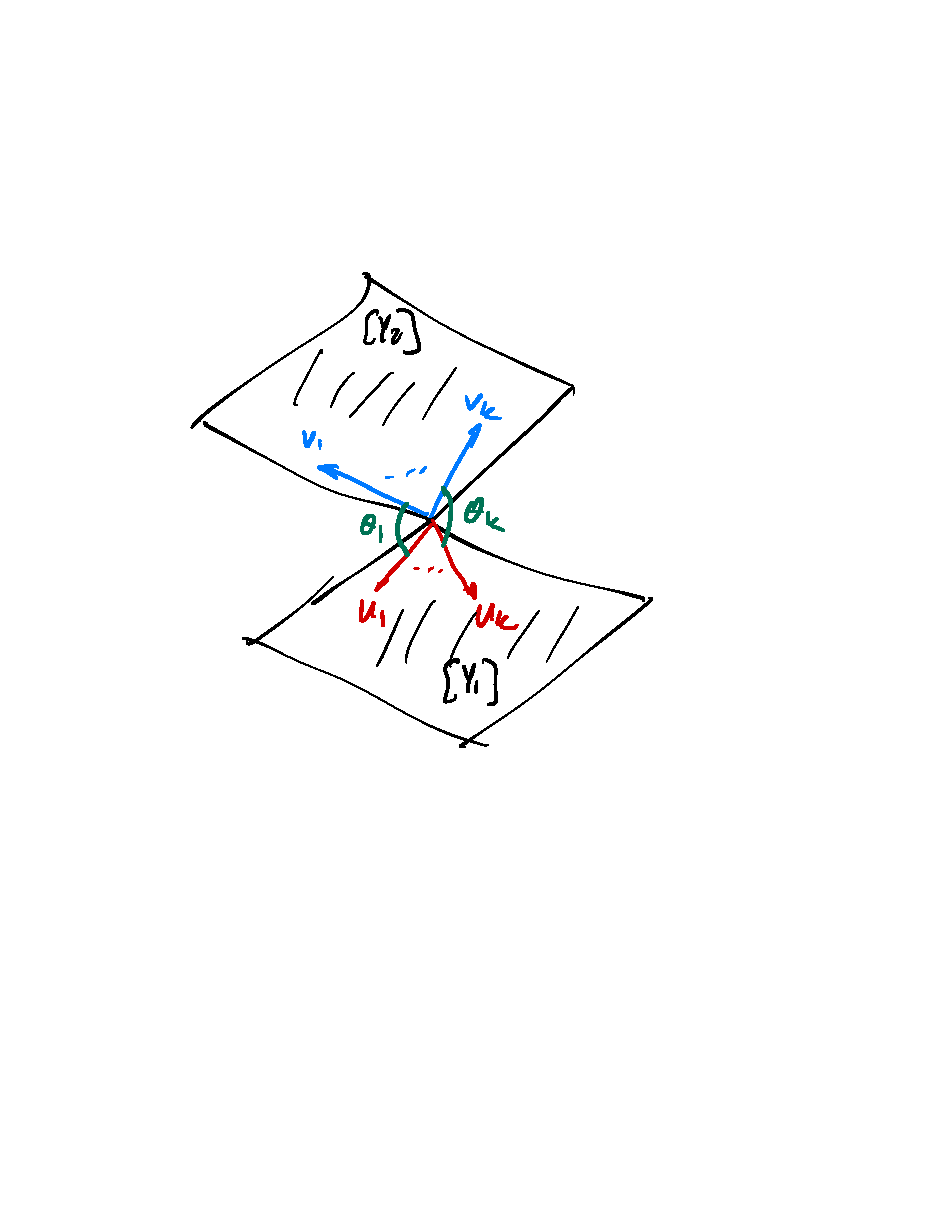
\includegraphics[height=1.5in]{principalangles}
	\caption{The aligned bases of two planes which realize the principal angles $\theta_1, \dots , \theta_k$ between the planes.}
	\alttext{Two planes sketched as rectangles at acute angles, together with arrows indicating basis vectors that realize the principal angles between the planes.}
	\label{fig:principal angles}
\end{figure}

And now, the geodesic from $[Y_1]$ to $[Y_2]$ is simple: 

\begin{theorem}\label{thm:grassmannian geodesics}
	Let $u_i(t)$ be the rotation of each $u_i$ to the corresponding $v_i$ at constant speed so that the angle between $u_i = u_i(0)$ and $u_i(t)$ is $t \theta_i$. This ensures that each $v_i = u_i(1)$. If $\gamma(t)$ is the subspace spanned by $u_1(t), \dots , u_k(t)$, which can be represented by the $n \times k$ orthonormal matrix $\begin{bmatrix} u_1(t) & \dots & u_k(t)\end{bmatrix}$, then $\gamma$ is a minimizing geodesic in $\Gr(k,\R^n)$ between $\gamma(0) = [Y_1]$ and $\gamma(1) = [Y_2]$.
\end{theorem} 

 
For example, $\Gr(1,\R^n) = \RP^{n-1}$ consists of lines through the origin, and this tells us that the geodesic between two lines is just the steady-speed rotation of one to the other.

	\ifplastex
	\begin{figure}[htbp]
		\centering
			\includegraphics[height=1.5in]{linegeo.gif}
		\caption{The geodesic between two lines in the plane.}
		\alttext{Two lines in the plane, one of which is stationary and the other of which rotates toward the first at a steady speed until they meet, at which point the motion is reversed.}
		\label{fig:line geodesics}
	\end{figure}
	\fi

\begin{example}	
In general, I can get random points in $\Gr(k,\R^n)$ by applying Gram–Schmidt to $n\times k$ matrices with standard Gaussian entries. 

	With $k=26$ and $n=57$ I generated $Y_1$ and $Y_2$ in this way; they're visualized in the first row of \Cref{fig:grassmannian points} by having the value in each entry specify a color. The second row of \Cref{fig:grassmannian points} shows the aligned representatives $Y_1U$ and $Y_2V$. Using \Cref{thm:distance in grassmannian}, $d([Y_1],[Y_2]) \approx 4.692$.
	
	\begin{figure}[htbp]
		\centering
			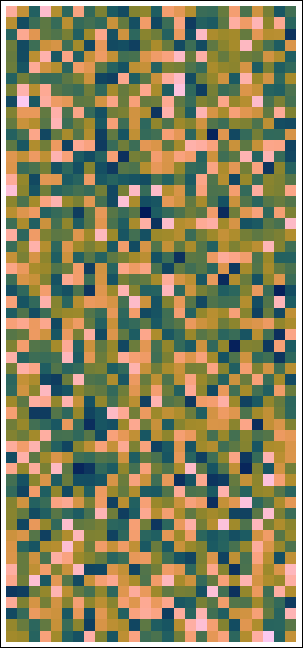
\includegraphics[height=1in]{grp1} \qquad \qquad 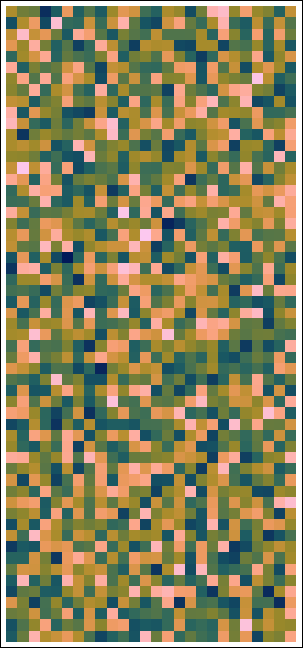
\includegraphics[height=1in]{grp2}
			
			\vspace{.2in}
			
			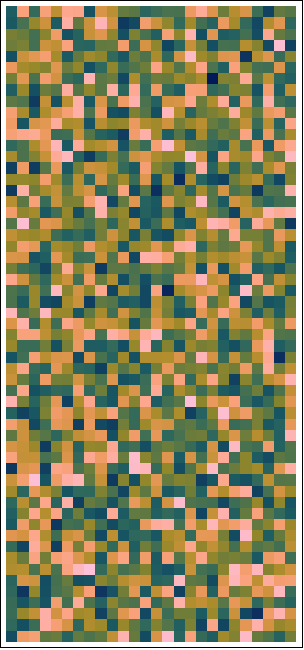
\includegraphics[height=1in]{grp1a} \qquad \qquad 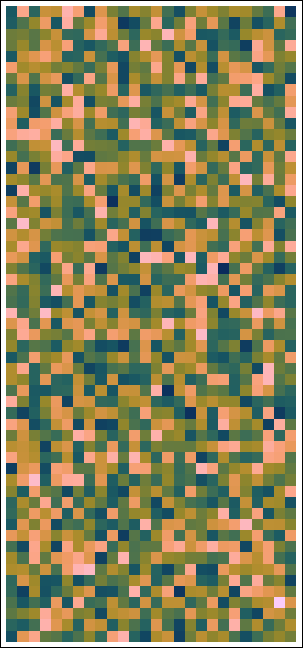
\includegraphics[height=1in]{grp2a}
		\caption{Two points in $\Gr(k,\R^n)$ represented by matrices visualized in the first row, with the aligned representatives visualized in the second row.}
		\alttext{Four matrix plots visualizing random $57 \times 26$ orthonormal matrices shown in a $2 \times 2$ grid. The entries in the same column correspond to the same point in the Grassmannian.}
		\label{fig:grassmannian points}
	\end{figure}
	
	In turn, \Cref{fig:grassmannian geodesic} shows a few equally-spaced points along the minimizing geodesic given by \Cref{thm:grassmannian geodesics} connecting these two points in the Grassmannian.
	
	\begin{figure}[htbp]
		\centering
			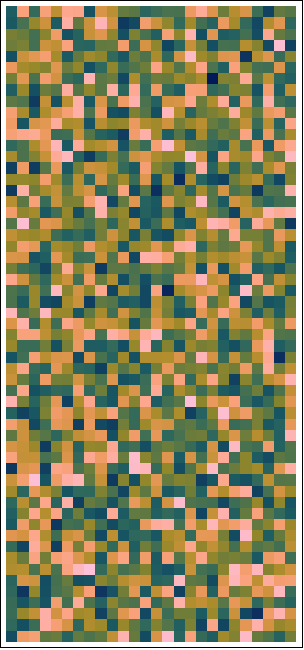
\includegraphics[height=1in]{grgeo1} \qquad 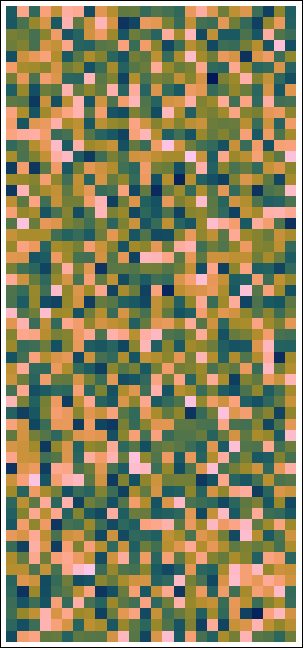
\includegraphics[height=1in]{grgeo11} \qquad 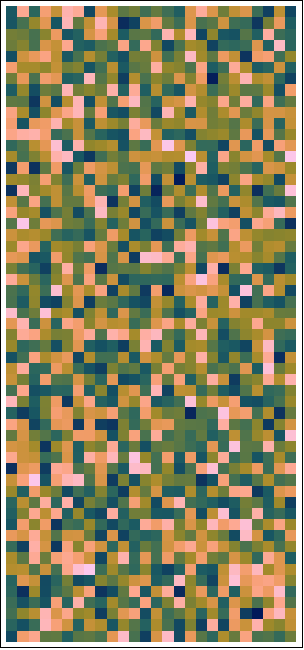
\includegraphics[height=1in]{grgeo21} \qquad 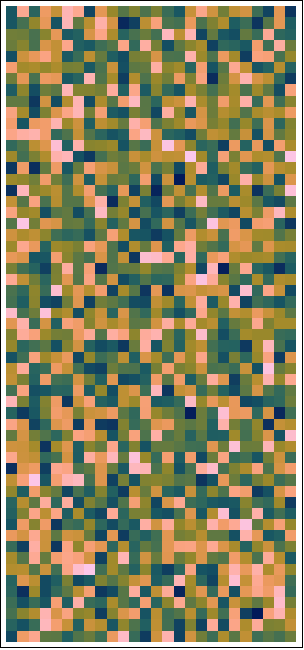
\includegraphics[height=1in]{grgeo31} \qquad 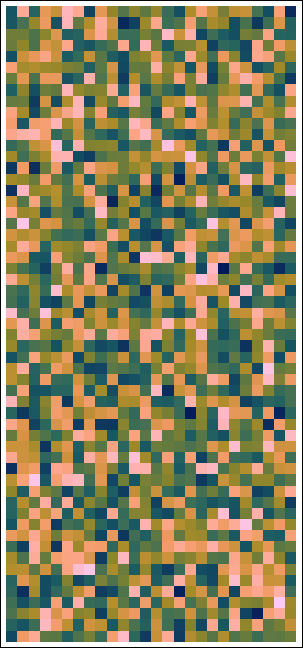
\includegraphics[height=1in]{grgeo41} \qquad 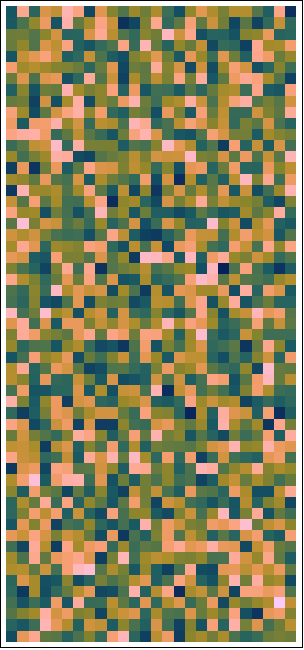
\includegraphics[height=1in]{grgeo51} \qquad 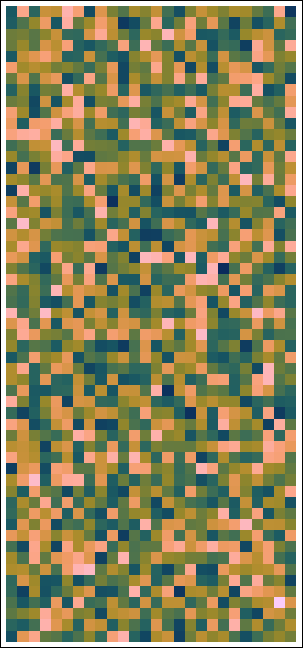
\includegraphics[height=1in]{grgeo61} 
		\caption{Seven equally-spaced points along the minimizing geodesic from $[Y_1]$ to $[Y_2]$ in $\Gr(26,\R^{57})$.}
		\alttext{Seven matrix plots in a row that visualized the geodesic described in the main text. They are visually all very similar.}
		\label{fig:grassmannian geodesic}
	\end{figure}
	
	Here is a video showing the full geodesic: 
	
	\vimeo{1078821889}
	
	Using \Cref{thm:distance in grassmannian} it is straightforward to compute distances between points in the Grassmannian. \Cref{fig:grassmannian distance histogram} shows the histogram of distances between 10,000 pairs of random points in $\Gr(26,\R^{57})$, which fits quite well to the Gaussian distribution with mean $4.844$ and standard deviation $0.0788$. Note that the maximum possible distance is $\sqrt{26}\frac{\pi}{2}\approx 8.0095$.
	
	\begin{figure}[htbp]
		\centering
			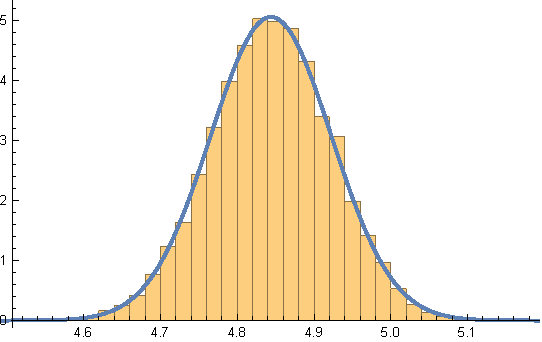
\includegraphics[height=1.5in]{grhist}
		\caption{Histogram of distances between 10,000 pairs of random points on $\Gr(26,\R^{57})$, together with the graph of the probability density function of the Gaussian distribution with mean $4.844$ and standard deviation $0.0788$.}
		\alttext{Histogram of data which is approximately normally distributed with values ranging between 4.5 and 5.2.}
		\label{fig:grassmannian distance histogram}
	\end{figure}
\end{example}